\section{Noise and Errors}
\label{sec:noise-errors}

This section analyzes the impact of noise on protocol variants that teleport either energy or charge. We model imperfections in the classical communication channel together with noise processes acting on the entangled resource state, specifically bit-flip, phase-flip, and contamination from excited states. Robustness is assessed under realistic error budgets via numerical studies and device-level simulations performed in \texttt{Qiskit}. Our emphasis is comparative: we contrast energy- and charge-teleportation across the star-coupled ($H^{(1)}$) and nearest-neighbor ($H^{(2)}$) models, referencing extended data in Appendix~\ref{appendix:noise-errors}.

A primary metric for protocol failure is the sign reversal of the teleported expectation value $\langle \Delta O_B \rangle$. Since the protocol encodes key bits in this sign, a flip from negative to positive constitutes a bit-error, rendering the key insecure. We analyze the error probability threshold at which such reversals occur, identifying the operational limits for reliable information transmission.

\subsection{Classical Communication Error}
\label{subsec:classical-comm}

\begin{figure}[ht]
  \centering
  \subfloat[\(H^{(1)}\) (Star-Coupling interaction)]{
        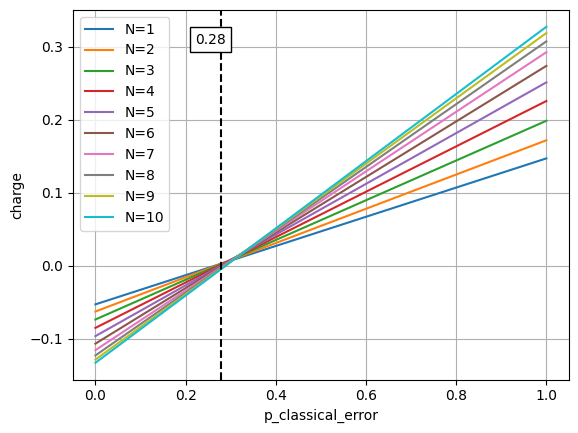
\includegraphics[width=0.8\columnwidth]{plots/errors/numerical/Alice_charge_vs_p_class_comm_err.png}
    }
  \vspace{0.5em}
  \subfloat[\(H^{(2)}\) (Nearest-Neighbors interaction), \(\sigma_A=X_0\)]{
        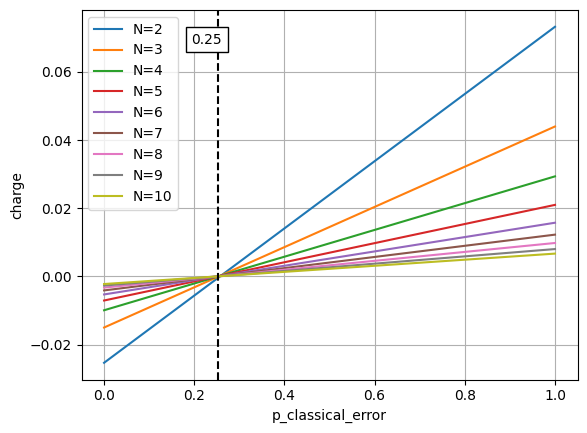
\includegraphics[width=0.8\columnwidth]{plots/errors/numerical/NN_X_charge_vs_p_class_comm_err.png}
    }
  \vspace{0.5em}
  \subfloat[\(H^{(2)}\) (Nearest-Neighbors interaction), \(\sigma_A=Y_0\)]{
        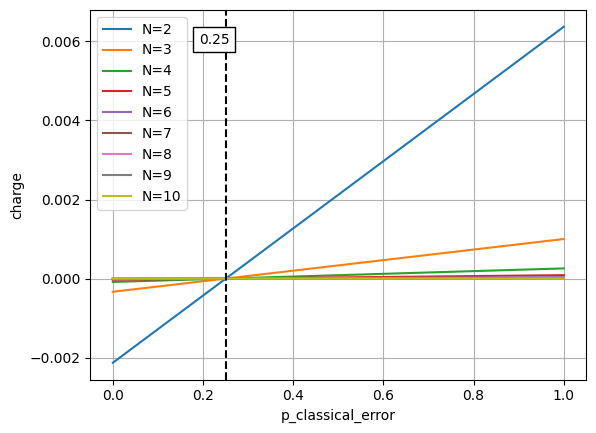
\includegraphics[width=0.8\columnwidth]{plots/errors/numerical/NN_Y_charge_vs_p_class_comm_err.png}
    }
  \caption{Classical communication error: numerical \(\langle \Delta O_B\rangle\) vs. classical communicated bit-flip probability \(p\) across multiple system sizes \(N\) for Charge. We see a consistent failure threshold around $p \approx 0.25-0.28$}
  \label{fig:cls-Ns-main}
\end{figure}

An error in the classical channel, where the bit Alice sends is flipped with probability $p$, causes Bob to apply the incorrect unitary operation. This effectively creates a statistical mixture of the intended ($a=0$) and flipped ($a=1$) outcomes. As analyzed in \cite{QKDbyQET}, this leads to a linear degradation of the expected signal: $\langle\Delta O_B\rangle_p = (1-p)\langle\Delta O_B\rangle_{a=0} + p\langle\Delta O_B\rangle_{a=1}$. Since $\langle\Delta O_B\rangle_{a=0}$ is negative and $\langle\Delta O_B\rangle_{a=1}$ is positive, the signal is attenuated and moves towards zero.

The numerical results in Figure~\ref{fig:cls-Ns-main} show this linear decay for all simulated configurations. For the star-interaction model $H^{(1)}$, a clear sign-flip threshold appears around $p \approx 0.25$, consistent with the findings in \cite{QKDbyQET}. While the absolute magnitude of the energy signal is larger than that of the charge signal in this model, both are similarly vulnerable to this error (see Appendix Fig.~\ref{fig:classical_err_alice_ham} and Fig.~\ref{fig:classical_err_nn_ham_x} for a direct comparison). However, for the more realistic nearest-neighbor model ($H^{(2)}$), the energy signal diminishes rapidly with system size $N$, whereas the charge signal remains more stable (a trend clearly visible in the energy data in Appendix Fig.~\ref{fig:energy_vs_classical_err_for_n}). This highlights that for larger distances, the charge protocol's signal is more resilient, even though the fundamental error threshold remains similar.

From Figure~\ref{fig:classical-main} one can see that error flipping the classical bit communicated from Alice to Bob changes the extracted value sign at Bob's site at high probabilities. This is the expected result since by the protocol's design and from simulations of the protocol in previous sections we showed that flipping this bit inverts the sign measured by Bob. Comparing to energy from the equivalence simulation in~\cite{QKDbyQET} (see also Figures~\ref{fig:classical_err_alice_ham},~\ref{fig:classical_err_nn_ham_x} and~\ref{fig:classical_err_nn_ham_y} in Appendix), the charge is somewhat more robust to such error where the sign flips around \(p_{err} \approx  0.32\) instead of \(p_{err} \approx  0.25\) for energy, a threshold introduce in~\cite{QKDbyQET} and is confirmed in our own energy teleportation simulations (Appendix Fig.~\ref{fig:classical_err_alice_ham}, Fig.~\ref{fig:classical_err_nn_ham_x} and Fig.~\ref{fig:classical_err_nn_ham_y}).

\begin{figure}[ht]
  \centering
  
\includegraphics[width=0.8\columnwidth]{plots/errors/numerical/N2_charge_vs_p_classical_error.png}
  \caption{Classical communication error for the $H^{(2)}$ model ($N=2, \sigma_A=X_0$). The sign-flips are
not prominent at low error probabilities.}
  \label{fig:classical-main}
\end{figure}

\subsection{Mixture with an Excited State}
\label{subsec:mixture}

\begin{figure}[ht!]
    \centering
    \subfloat[Numerical, \(H^{(2)}\), \(N{=}2\), \(\sigma_A=X_0\)]{
        
\includegraphics[width=0.8\columnwidth]{plots/errors/numerical/N2_charge_vs_p_excited_mixture_error.png}
    }
    \vspace{0.5em}
    \subfloat[Qiskit, \(H^{(2)}\), \(N{=}2\), \(\sigma_A=X_0\)]{
        
\includegraphics[width=0.9\columnwidth]{plots/errors/qiskit/N2_charge_vs_p_excited_mixture_error.png}
    }
  
  \caption{Mixture with an excited state for the $H^{(2)}$ model ($N=2, \sigma_A=X_0$). For most \(J\) values, the signal remains negative, demonstrating its robustness. Qiskit simulations (bottom) confirm the trend but show higher statistical variance.}
  \label{fig:mixture-main}
\end{figure}

Perfect ground state preparation is experimentally challenging; a common imperfection is a residual population of excited states, modeled as a classical mixture $\rho = (1-p)\rho_{gs} + p\rho_{excited}$. The teleported signal becomes a weighted average of the contributions from each state.

Figure~\ref{fig:mixture-main} reveals a critical performance difference between energy and charge teleportation.
This difference in robustness stems from the nature of the observables themselves. The energy teleportation signal is highly sensitive to the local energy expectation value $\langle H_B\rangle$. Low-lying excitations contribute a large positive energy offset, which can easily overwhelm the negative teleported signal originating from the ground state component, causing a premature sign-flip fatal to the QKD protocol.

% This is part of the next subsection of superposition with excited state error, it is here for formatting resons
\begin{figure*}[htbp]
    \centering
    \subfloat[Numerical, \(H^{(2)}\), \(N{=}2\), \(\sigma_A=X_0\)]{
        
\includegraphics[width=0.8\columnwidth]{plots/errors/numerical/N2_charge_vs_p_excited_superposition_error.png}
    }
    \hfill
    \subfloat[Qiskit, \(H^{(2)}\), \(N{=}2\), \(\sigma_A=X_0\)]{
        
\includegraphics[width=0.9\columnwidth]{plots/errors/qiskit/N2_charge_vs_p_excited_superposition_error.png}
    }
  
  \caption{Coherent superposition with an excited state for the $H^{(2)}$ model ($N=2, \sigma_A=X_0$). Similar to the classical mixture, the charge protocol proves its resilient.}
  \label{fig:superposition-main}
\end{figure*}

In contrast, the charge observable $Q_B$, which is related to local spin parity, is less sensitive to these absolute energy shifts. The quantum correlations responsible for generating the signal's sign (the $\eta_Q$ term) often retain their structure across different low-energy states. As a result, the contribution from the excited state does not introduce a large positive offset, and the teleported charge signal remains negative over a much wider range of error probabilities, merely decreasing in magnitude.
While both signals degrade as the mixture probability $p$ increases, the energy signal frequently crosses zero and becomes positive at moderate error levels ($p \approx 0.15-0.25$) \cite{QKDbyQET}, a critical vulnerability that is evident in our energy simulations shown in Appendix Fig.~\ref{fig:nn_X_num_mixture_error_appendix} and Fig.~\ref{fig:nn_Y_num_mixture_error_appendix}. In contrast, the charge signal often remains negative even at high error probabilities, merely decreasing in magnitude. This superior robustness of charge stems from the nature of the observables - because charge is related to symmetry which is preserved in low-lying excitations, whereas energy is directly corrupted by the excitation gap. Low-lying excitations can significantly alter the local energy expectation value $\langle H_B \rangle$, contributing a large positive offset term ($\xi_H$) that overwhelms the negative teleported signal from the ground state. The charge observable $Q_B$, which is tied to local spin parity, is less sensitive to such energy shifts. The correlations responsible for charge teleportation ($\eta_Q$) often retain their sign across different low-energy manifolds, preserving the integrity of the key bit.

The Qiskit simulations (top panels of Fig.~\ref{fig:mixture-main}) corroborate these findings while also illustrating the practical measurement challenges. The energy plots exhibit significant statistical variance, a direct result of the weak signal and the error propagation from measuring non-commuting terms (Appendix~\ref{appendix:stats-analysis}). The charge plots are markedly smoother, underscoring not only its theoretical robustness but also its superior statistical stability in a measurement context. This trend holds across all tested Hamiltonians and system sizes, as detailed in Appendix~\ref{appendix:noise-errors}.

\subsection{Superposition with an Excited State}
\label{subsec:superposition}

A coherent error creating a superposition $|\psi\rangle = \sqrt{1-p}|\psi_{gs}\rangle + e^{i\alpha}\sqrt{p}|\psi_{excited}\rangle$ introduces interference terms into the expectation values of $\xi$ and $\eta$. This leads to a non-linear dependence on the error probability $p$, as shown in Figure~\ref{fig:superposition-main}. Similar to the classical mixture, the energy protocol is more susceptible to sign-flips than the charge protocol, as shown in the energy data in Appendix Fig.~\ref{fig:nn_X_num_superposition_error_appendix} and Fig.~\ref{fig:nn_Y_num_superposition_error_appendix}. The phase sensitivity inherent in the superposition can destructively interfere with the commutator term $\eta$, which is the engine of teleportation, and this effect appears more pronounced for the energy observable. The Qiskit simulations again highlight the increased statistical variance, making it difficult to distinguish the true non-linear signal from finite-shot noise.

\subsection{Bit-Flip and Phase-Flip Errors}
\label{subsec:quantum-channel-errors}

\begin{figure}[ht!]
    \centering
    \subfloat[Numerical, \(H^{(2)}\), \(N{=}2\), \(\sigma_A=X_0\)]{
        
\includegraphics[width=0.8\columnwidth]{plots/errors/numerical/N2_charge_vs_p_bitflip_error.png}
    }
    \vspace{0.5em}
    \subfloat[Qiskit, \(H^{(2)}\), \(N{=}2\), \(\sigma_A=X_0\)]{
        
\includegraphics[width=0.9\columnwidth]{plots/errors/qiskit/N2_charge_vs_p_bitflip_error.png}
    }
  
  \caption{Bit-flip error on the resource state for the $H^{(2)}$ model ($N=2, \sigma_A=X_0$). We see a smooth, gradual degradation without a sharp sign-crossing threshold, indicating relative robustness against this error type.}
  \label{fig:bitflip-main}
\end{figure}

\begin{figure*}[ht!]
    \centering
    \subfloat[Numerical, Alice's site]{
        
\includegraphics[width=0.4\textwidth]{plots/errors/numerical/N2_charge_vs_p_alice_phaseflip_error.png}
    }
    \hfill
    \subfloat[Qiskit, Alice's site]{
        
\includegraphics[width=0.55\textwidth]{plots/errors/qiskit/N2_charge_vs_p_alice_phaseflip_error.png}
    }

    \vspace{0.5em}
  
    \subfloat[Numerical, Bob's site]{
        
\includegraphics[width=0.4\textwidth]{plots/errors/numerical/N2_charge_vs_p_bob_phaseflip_error.png}
    }
    \hfill
    \subfloat[Qiskit, Bob's site]{
        
\includegraphics[width=0.55\textwidth]{plots/errors/qiskit/N2_charge_vs_p_bob_phaseflip_error.png}
    }

  \caption{Phase-flip error for the $H^{(2)}$ model (with $N=2, \sigma_A=X_0$). On Alice's site, the error attenuates the signals by decohering the measurement basis, but sign-flips are not prominent at low error probabilities. On Bob's site, the error is more detrimental, causing a rapid decay by inverting Bob's conditional rotation.}
  
  \label{fig:phaseflip-main}
\end{figure*}

We now consider local quantum channel noise acting on individual qubits.

\paragraph{Bit-Flip Error ($X_n$).} This error, modeled by $\rho \rightarrow (1-p)\rho + pX_n\rho X_n$, degrades the specific quantum correlations leveraged by the protocol. As shown in Figure~\ref{fig:bitflip-main}, both energy and charge signals decay smoothly with the error probability $p$. Sign-crossings are rare, indicating that the protocol is relatively robust against this error type. Energy generally maintains a larger absolute signal, which in principle makes it easier to measure, provided the noise level is low enough to prevent ambiguity (cf. the energy data in Appendix Figs.~\ref{fig:alice_num_bitflip_error_appendix},~\ref{fig:nn_X_num_bitflip_error_appendix}, and~\ref{fig:nn_Y_num_bitflip_error_appendix}).

\paragraph{Phase-Flip Error ($Z_n$).} The impact of a phase-flip error depends critically on its location.

\begin{itemize}
    \item \textbf{On Alice ($Z_0$):} A phase flip on Alice's qubit prior to her measurement effectively decoheres her measurement basis (since $\{Z_0, X_0\}=0$ and $\{Z_0, Y_0\}=0$). This directly suppresses the commutator term $\eta=i\langle[O_B, \sigma_B]\sigma_A\rangle$, thereby attenuating the teleported signal, a behavior observed for both charge (Fig.~\ref{fig:phaseflip-main}) and energy (Appendix Figs.~\ref{fig:nn_X_num_alice_phaseflip_error_appendix} and~\ref{fig:nn_Y_num_alice_phaseflip_error_appendix}).
    \item \textbf{On Bob ($Z_N$):} A phase flip on Bob's qubit is more detrimental. Since Bob's unitary operation is typically a rotation around the Y or X axis, the transformation $Z_N R_Y(\theta) Z_N^\dagger = R_Y(-\theta)$ shows that a phase flip inverts the sign of his rotation. This is equivalent to receiving a flipped classical bit from Alice and causes a rapid linear decay that accelerates the protocol's failure, an effect that is equally detrimental to the charge (Fig.~\ref{fig:phaseflip-main}) and energy (Appendix Figs.~\ref{fig:alice_num_bob_phaseflip_error_appendix},~\ref{fig:nn_X_num_bob_phaseflip_error_appendix} and~\ref{fig:nn_Y_num_bob_phaseflip_error_appendix}).
\end{itemize}

In both cases, energy and charge show similar qualitative degradation, although the protocol is clearly more sensitive to noise on Bob's side.

% This belongs to the next subsection, it is here for formatting reasons
\begin{table*}[t]
\small
\centering
\caption{Qualitative comparison of teleported \textbf{energy} (E) vs.\ \textbf{charge} (Q) under various noise channels. The assessment is based on trends observed across different Hamiltonians and system sizes.}
\label{tab:noise-summary-improved}
\begin{tabularx}{\textwidth}{@{} l >{\hsize=0.8\hsize}X >{\hsize=0.8\hsize}X >{\hsize=1.4\hsize}X @{}}
\toprule
\textbf{Error Type} & \textbf{Signal Strength (E vs. Q)} & \textbf{Sign-Crossing (E vs. Q)} & \textbf{Dominant Physical Mechanism} \\
\midrule
Classical Comm. Error & E typically larger, but decays faster with N in $H^{(2)}$ & High for both at $p \approx 0.25-0.5$ & Linear mixing of the two classical ($a=0, 1$) branches, as predicted in \cite{QKDbyQET}. \\
\addlinespace
Mixture w/ Excited State & Both decay. E signal degrades faster & High risk for E; Very low for Q & E is highly sensitive to local energy offsets ($\xi_H$) of excited states. Q's sign (from $\eta_Q$) is more robust across low-energy manifolds. \\
\addlinespace
Superposition w/ Excited & Both decay non-linearly & High risk for E; Low for Q & Interference terms renormalize $\eta$ and $\xi$. This effect is more detrimental for the energy protocol. \\
\addlinespace
Bit-Flip Error (X) & E typically maintains a larger signal & Low for both & General degradation of the quantum correlations needed for teleportation. Requires high $p$ to cause sign-flip. \\
\addlinespace
Phase-Flip on Alice (Z) & E typically maintains a larger signal & Low for both & Decoheres Alice's measurement basis ($X_0/Y_0$), which attenuates the commutator term $\eta$ responsible for signal generation. \\
\addlinespace
Phase-Flip on Bob (Z) & Both decay rapidly & Moderate for E; Low for Q & Inverts the sign of Bob's rotation ($R_Y(\theta) \to R_Y(-\theta)$), which mimics a classical bit-flip and accelerates signal decay. \\
\bottomrule
\end{tabularx}
\end{table*}

\subsection{Energy vs. Charge: A Consolidated View}
\label{subsec:consolidated}

Our analysis reveals a consistent trade-off between energy and charge teleportation. \textbf{Energy teleportation} can yield a stronger absolute signal, especially for the directly-coupled star Hamiltonian ($H^{(1)}$). However, this larger signal comes at the cost of fragility. Energy is fundamentally sensitive to errors that shift local energy offsets, such as contamination from excited states, which can induce premature sign-flips that are fatal to a QKD protocol. Moreover, its practical implementation is hampered by higher statistical noise arising from the need to measure non-commuting observables separately (Appendix~\ref{appendix:stats-analysis}).

In contrast, \textbf{charge teleportation} offers a more stable and robust signal. While its magnitude is often smaller, its resilience against sign-flips—particularly under excited-state mixture—is a decisive advantage. This robustness, combined with its perfect symmetry and superior statistical clarity from single-operator measurements, makes it a more reliable and scalable choice. These qualities are especially critical for the nearest-neighbor model, where the signal is inherently weaker and decays with distance, making the statistical stability of charge a key enabler. Table~\ref{tab:noise-summary-improved} summarizes these comparative findings.

Collectively, these results strongly suggest that the stability and resilience of charge teleportation make it a more promising candidate for the practical implementation of observable-based QKD on near-term quantum devices.

\medskip
\noindent\emph{Note.} Additional configurations, including extended \(N\) sweeps and further comparisons, are introduced in Appendix~\ref{appendix:noise-errors} for completeness.
